\section{Evaluation}
We show the evaluation of four existing basic block-level
performance models on three recent Intel microarchitecture:
Ivy Bridge, Haswell, and Skylake. Furthermore we discuss a few basic blocks where most models
mis-predict by more than~30\%.

For the Ivy Bridge measurements,
we used a server with the Intel(R) Xeon(R) CPU E5-2695 v2 CPU and 128 GBs of memory. 
For the Haswell measurements,
we used a server with the Intel(R) Xeon(R) CPU E5-2680 v3 CPU and 128 GBs of memory. 
Finally, for the Skylake measurements, we used a server with the Intel(R) Xeon(R) W-2123 CPU and 64 GBs of memory. 

We evaluated IACA~\cite{iaca}, llvm-mca~\cite{llvm-mca}, Ithemal\cite{ithemal}, and OSACA\cite{osaca}
on three recent Intel microarchitectures: Ivy Bridge, Haswell, and Skylake.
Some basic blocks in our dataset contain AVX2 instructions,
which are not implemented in Ivy Bridge,
and these basic blocks are not included in the Ivy Bridge evaluation.
For Skylake and Haswell, we used IACA 3.0;
and for Ivy Bridge we used IACA 2.0, because IACA discontinued its support for
Ivy Bridge after version 2.0.
For llvm-mca, we used version 9.0.0.
OSACA is currently under development and we took the latest version
at the time of writing this paper.
For Ithemal too, we contacted the authors and obtained the latest version from them.

We use relative error (defined in Equation~\ref{eq:rel_err}, where $t$ is the measured throughput and $t'$ is the throughput predicted by a model)
as the main metric to measure inaccuracy.
We use error and relative error interchangeably in the rest of the paper.
We additionally evaluated how each model preserves ordering of basic block performance,
using Kendall's tau coefficient~\cite{kendalltau},
which measures the fraction of preserved pairwise ordering.
\begin{equation}
\mathit{err}(t, t') = \left| \frac{t - t'}{t'} \right| 
\label{eq:rel_err}
\end{equation}

\subsection{Evaluation Metrics}\label{results}
We report the prediction errors of the performance models in three different ways.

\textbf{Overall error} This is the unweighted average error for all basic blocks.
Table \ref{tab:overall} shows the overall error of each model on different microarchitectures.
We note that the overall error of each model can be unrepresentative
of its performance on a given domain.
We additionally compute the Kendall's tau coefficients~\cite{kendalltau} for the models;
this coefficient measures the fraction of throughput ordering
preserved by performance modelling.
Kendall's tau coefficient is interesting when the consumers of a performance model
are not so much concerned with the precise predictions but
the relative ordering of predictions--such as compiler optimizations that needs 
to select the best of candidate programs.

\textbf{Per-application error}
For each application, we weight its basic blocks by their approximate
dynamic execution frequency,
and report the weighted average error.
We obtain each basic block's dynamic frequency using sample-based profiling.
Weighting the basic blocks allows us to focus on those that have
non-negligible effects on performance.
Most basic blocks collected from TensorFlow\cite{tensorflow},
for instance, are from infrequently executed code 
such as the Python interpreter or glibc;
weighting these basic blocks allows a user of the benchmark
to see an evaluation  of the performance model relevant
to the application's expected runtime cost.
Figures \ref{fig:ivb-app-err}, \ref{fig:hsw-app-err}, and \ref{fig:skl-app-err}
show the breakdown of the errors by applications.

\textbf{Per-category error} 
We automatically classify the basic blocks into
to different categories, as presented in Section~\ref{classification},
and report the average error for each category.
Using per-category error complements per-application error,
because the weighted average error for an application can be less informing 
when the application is dominated by a few basic blocks
(i.e. Eigen, Tensorflow, and Gzip).
Figure \ref{fig:ivb-cluster-err}, \ref{fig:hsw-cluster-err}, 
and \ref{fig:skl-cluster-err} show the breakdown of the errors by basic block categories.

The discrepancy between overall unweighted accuracy (Table ~\ref{tab:overall})
and that of more specialized types of basic blocks
such as vectorized code (Figures \ref{fig:ivb-cluster-err},
\ref{fig:hsw-cluster-err},
and \ref{fig:skl-cluster-err}) highlights
the need of basic block classification and per-category error reporting.

\subsection{Analysis}
 %We first analyze how accurate and stable each estimation method is considering all error metrics. Next, we analyze per-application and per-category errors on how they differ across various microarchitectures for different estimation methods.\\
 
%We analyze the performance of IACA, llvm-mca, Ithemal, and OSACA.
 
 \textbf{IACA}~\cite{iaca} is relatively stable compared to other models that we evaluated.
An interesting point to note is that IACA is consistently accurate on basic blocks from OpenSSL. 
OpenSSL is a crypto library that is dominated by basic blocks containing vector and scalar operations
(category-1) and IACA models these well. 

    \textbf{llvm-mca}~\cite{llvm-mca} is considerably worse on all microarchitectures compared to IACA and Ithemal,
especially on modelling basic blocks involving loads. Also, the per-application error increases on recent microarchitectures like Skylake and Haswell compared to Ivy Bridge.
%We suspect the decrease in performance is a result of LLVM developers 
%having less time to update the cost models for the relatively new microarchitectures. 

\textbf{Ithemal}~\cite{ithemal} consistently outperforms other models, except on vectorized basic blocks (e.g. category-2).
Ithemal is also considerably better than other models at modelling basic blocks with memory dependence,
as demonstrated by its errors on predicting basic blocks from categories 4 and 8.
We discussed Ithemal's underperformance on vectorized basic blocks with the authors of Ithemal, who suggested that the inconsistency
was a result of imbalance in their training dataset;
the majority of which, similar to our data set, consists of non-vectorized basic blocks.

\textbf{OSACA}\cite{osaca} is on average more accurate than llvm-mca but
considerably less than IACA~\cite{iaca} and Ithemal~\cite{ithemal}.
We note that this has less to do with OSACA's methodology than the engineering of its currently under developement instruction parser.
During our evaluations, we found and reported five bugs related to OSACA's instruction parser.
In particular, OSACA does not recognize several instruction forms;
depending on the cases, it either crashes or treats unrecognized instruction forms as nops.
One such instruction form is any instruction that reads an immediate operand and writes to memory
(e.g. \verb|add $1, (rbx)|), and OSACA treats these instructions as nops, thus under-reporting the throughput of
many basic blocks.

\if 0
\textbf{Per-application error.} It is seen that per-application error for Haswell microarchitecture is worse for all estimation methods and it is especially prominent in llvm-mca~\cite{llvm-mca}. Also, note that OpenBLAS has significantly worse performance on Skylake for all analytical prediction methods. OpenBLAS contains lot of vectorized numerical kernels. We hypothesize that vector implementations in Skylake are different from older generations and are not modelled properly by the analytical estimation tools. Ithemal shows worse yet  similar performance on all microarchitectures for OpenBLAS. This may be because of the distributional bias in the training data of Ithemal.

\textbf{Per-category error.} Generally speaking, basic blocks dominated by stores
(category-4) are easier to predict,
while the throughput of basic blocks that mixes load instructions
with other operations (e.g. category-3) are considerably
more difficult to predict -- the prediction error is on average more than
twice higher than predicting basic blocks with only stores. 
We surmise that this is due to weakness of existing analyzers to model 
memory dependence.
In addition to basic blocks with memory dependence,
vectorized basic blocks (i.e. parts of category-1 and category-2) also cause high prediction errors.
\fi
% TODO summarize error by applications



\begin{table}
\begin{tabular}
{|p{0.25\columnwidth}|p{0.25\columnwidth}|p{0.15\columnwidth}|p{0.15\columnwidth}|}
\hline

\textbf{Microarchitecture} & \textbf{Model} &
\textbf{Average Error} & \textbf{Kendall's Tau Coefficient} \\
\hline

Ivy Bridge & IACA & 0.1664 & 0.8000\\
    & llvm-mca & 0.2813 & 0.7544\\
    & Ithemal & 0.1151 & 0.8296\\
    & OSACA & 0.3299 & 0.6197\\
\hline

Haswell & IACA & 0.1790 & 0.8043\\
    & llvm-mca & 0.2511 & 0.7829\\
    & Ithemal & 0.1200 & 0.8382\\
    & OSACA & 0.3566 & 0.6067\\
    
\hline 
Skylake & IACA & 0.1562 & 0.8066\\
    & llvm-mca & 0.2632 & 0.7693\\
    & Ithemal & 0.1146 & 0.8430\\
    & OSACA & 0.3433 & 0.5976\\

\hline
% TODO more for IVB and SKL
\end{tabular}
\\
\caption{Overall error of evaluated models. Kendall's tau coefficient~\cite{kendalltau}
measures the fraction of pairwise throughput ordering preserved by a given model.}
\label{tab:overall}
\end{table}


\begin{figure} 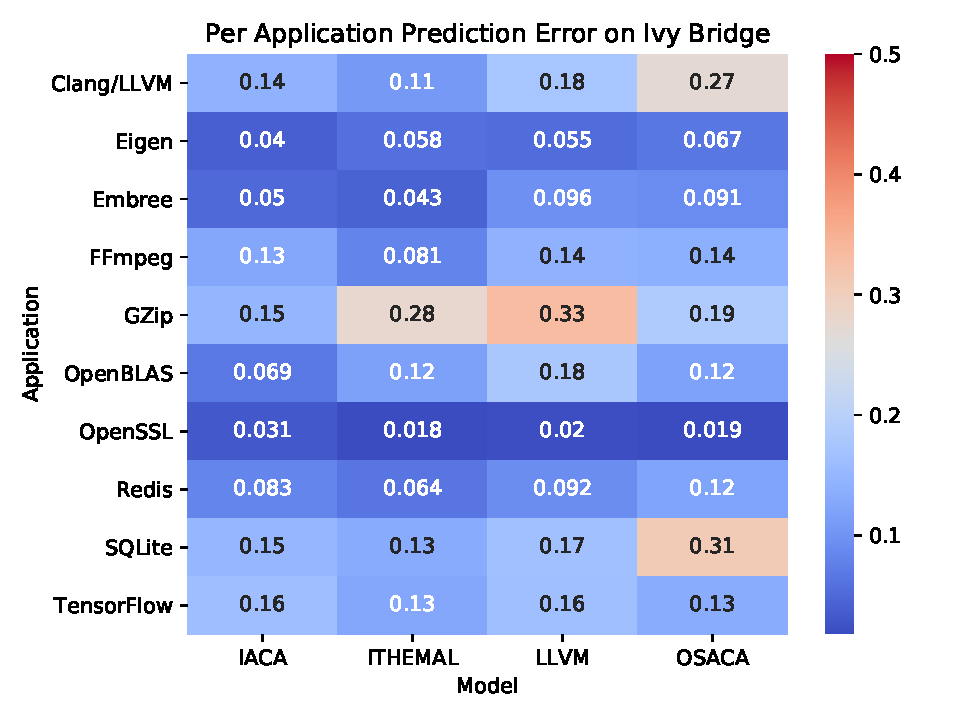
\includegraphics[width=\columnwidth]{figures/ivb-app-err.pdf} \caption{Per-application error for each model on Ivy Bridge;
error for each basic block is weighted by the frequency it is sampled during profiling.}
\label{fig:ivb-app-err}
\end{figure}

\begin{figure}
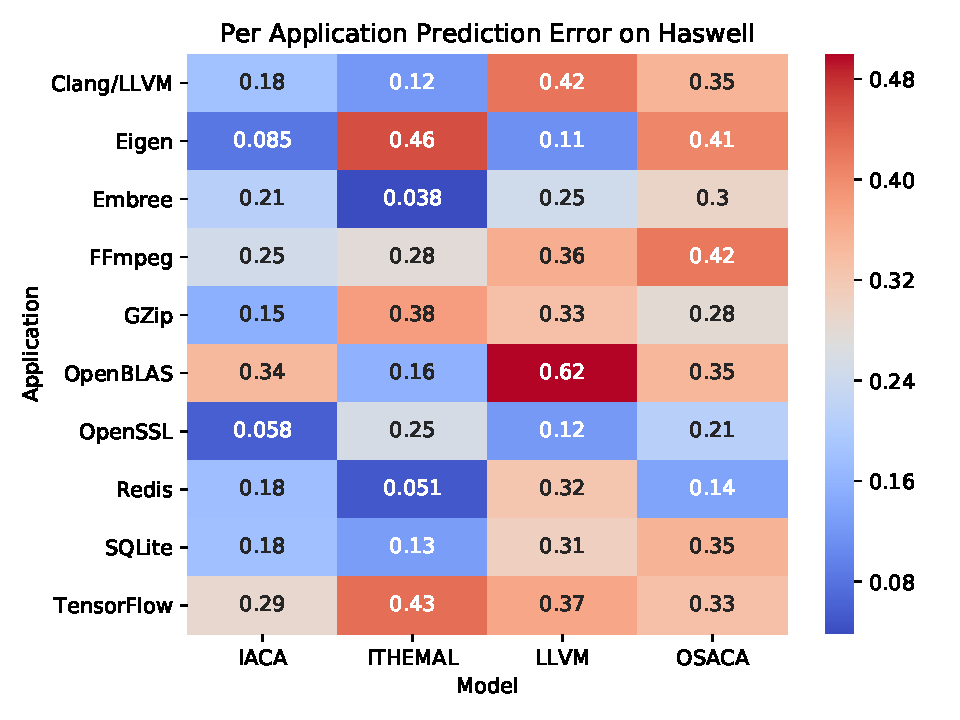
\includegraphics[width=\columnwidth]{figures/hsw-app-err.pdf}
\caption{Per-application error for each model on Haswell}
\label{fig:hsw-app-err}
\end{figure}

\begin{figure}
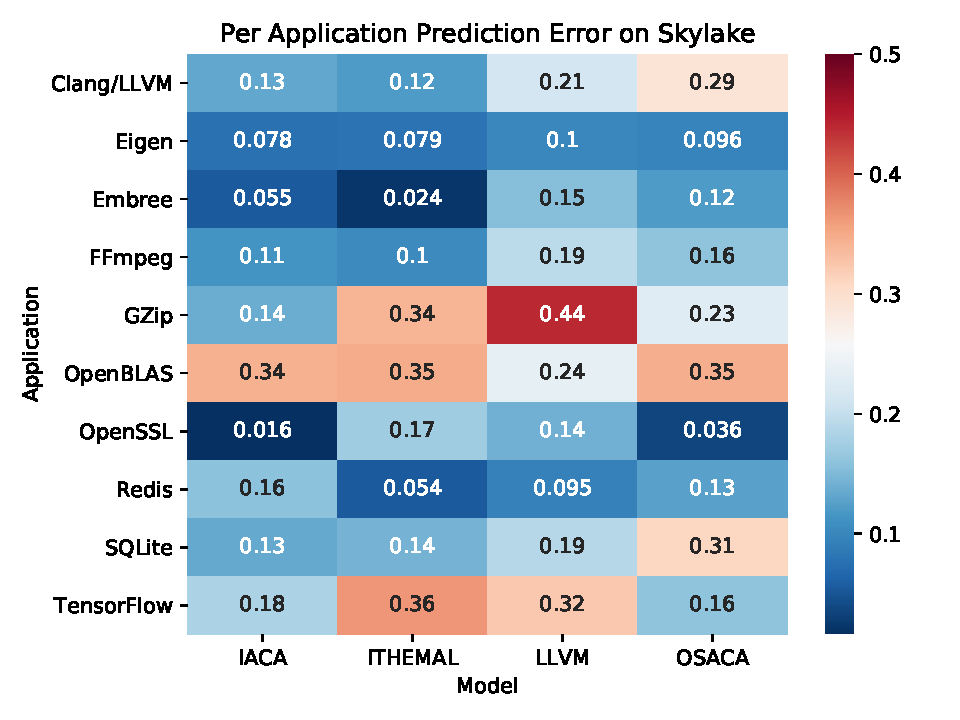
\includegraphics[width=\columnwidth]{figures/skl-app-err.pdf}
\caption{Per-application error for each model on Skylake. }
\label{fig:skl-app-err}
\end{figure}

\begin{figure}
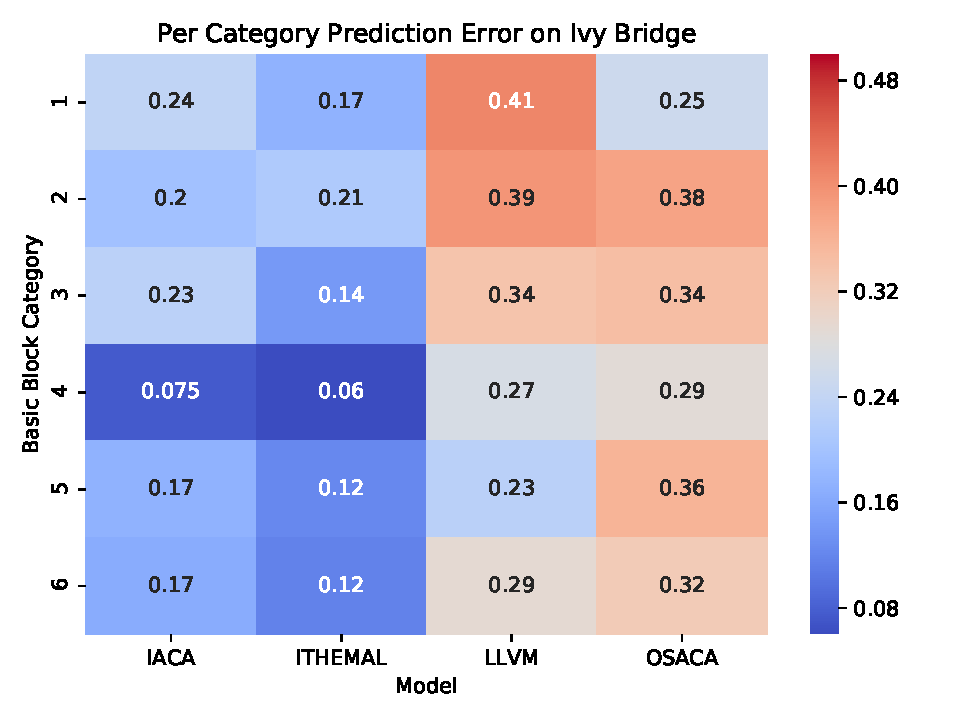
\includegraphics[width=\columnwidth]{figures/ivb-cluster-err.pdf}
\caption{Per-cluster error for each model on Ivy Bridge}
\label{fig:ivb-cluster-err}
\end{figure}

\begin{figure}
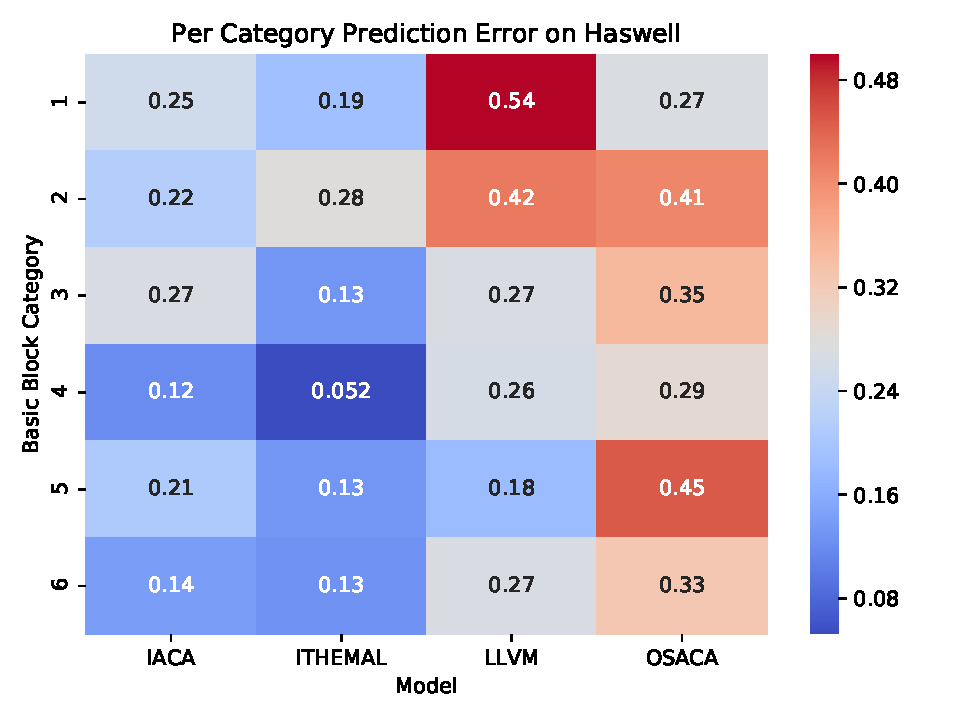
\includegraphics[width=\columnwidth]{figures/hsw-cluster-err.pdf}
\caption{Per-cluster error for each model on Haswell}
\label{fig:hsw-cluster-err}
\end{figure}

\begin{figure}
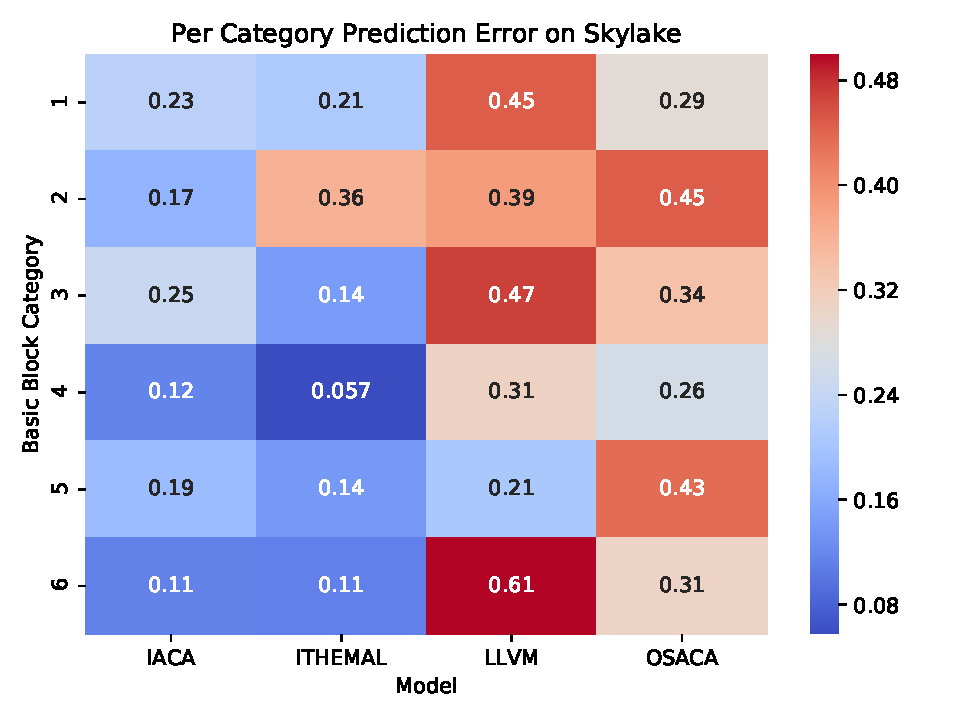
\includegraphics[width=\columnwidth]{figures/skl-cluster-err.pdf}
\caption{Per-cluster error for each model on Skylake}
\label{fig:skl-cluster-err}
\end{figure} 
